\section{緒論}
\subsection{背景}
近年來數據以飛快的速度成長,TB或是PB等級的數據隨處可見,在這資料快速產生且數據快速交換的時代,大數據一詞也越常被提及,國際數據公司(International Data Corporation, IDC)有研究指出,2008年全球生產的資料量為0.49ZB,2009年全球產生的資料量為0.8ZB,2010年增長為1.2ZB,2011年的資料量更是已經達到1.82ZB,這相當於全球每人生產200GB的資料,這麼龐大的資料也成了產業界與學術界所需要探討的重要議題,而有這麼大量的資料也意味著會有大量的應用會產生,而這一些應用當中一定會需要資料的交換,而在教會資料的時候,大多數的應用會選擇XML。\\\par
在大數據中,有所謂的5V,所謂的5V是指Volume, Value, Veracity, Vleocity, Variety,Volume是指產生的資料量;Value是指資料的價值;Veracity是指資料的可信度或是真實度;Velocity是指資料產生的速度;Variety是指資料的多樣性。而大數據在做資料交換的時候我們所關心的是資料的可信度或是真實度,也就是上述所提到的Veracity,這會影響到我們在做資料分析的結果可信度,假使進來的資料不具可信度的話,那麼所分析出來的結果自然也就不具有任何價值,本研究基於Apache Spark建構XML Veacity 真實度模型,利用Apache Spark 分散式大數據處理引擎,來計算並建構大型XML文件的Veracity 模型,並計算串流或批次輸入文件的Veracity 真實度評分。
\subsection{XML}
可延伸標記式語言(Extensible Markup Language,簡稱XML),是一種作為資料交換的結構化資料格式,XML是從標準通用標記式語言(SGML)中簡化修改出來的,XML是從1995年開始有雛形,並向全球資訊網聯盟(World Wide Web Consortium,簡稱W3C)提案,而在1998年2月發布為W3C的標準(XML 1.0)。\\\par
XML的特色在於文件內的標籤名稱可以由使用者自行定義,而XML文件必須是結構完整的(well-formed),所謂的well-formed是指XML除了要符合每一個標籤都要有起始元素之巢狀結構之外,還要符合格式規範,在XML中我們為了確保文件的格式正確性,會使用DTD(Document Type Definition)或是XML Scheme,DTD是XML提供的文件驗證機制,這是用來定義文件合法區塊,也就是定義元素的架構,有使用DTD的XML都必須依照DTD所定義的格式來呈現,下面是一個使用DTD且well-formed的XML文件範例:
\lstinputlisting[language=XML, frame=single]{example.xml}
但由於XML DTD並不能完全滿足XML自動化處理的要求,也缺乏對於文件結構屬性和資料屬性的規範,所以W3C在2001年的時候提出XML Schema,XML Schema使用的語法與XML相同,且支援四十多種資料類型,下面是一個使用XML Schema且使用此Schema驗證的XML文件範例:
\newpage
\lstinputlisting[language=XML, frame=single]{john.xml}
\lstinputlisting[frame=single]{business.xsd}
\par
上面有提到大數據資料真實度的重要性,假設資料缺乏真實度或是可信度,將增加資料處理的負擔,所以判斷資料的真實度是十分重要的事情,而要對大數據資料或是大型XML做資料真實度判斷有以下兩點困難
\begin{enumerate}
\item 資料來源多元且格式各異,有些XML有使用DTD,有些沒有,再來是XML標籤名稱是可以自行指定的,所以導致XML的資料格式不一。
\item 假設我們要求資料的一致性,那麼我們在資料進入系統的時候必須做資料清洗的動作,但是在大數據的資料或是大型XML的資料規模巨大,所以必須耗費大量的時間在資料清洗上面,在處理速度和資料真實度之間取捨,資料分析之後的結果要能夠呈現出資料的真實度以及可信度,所以真實度的重要性可想而知。
\end{enumerate}
\par
根據上述原因,XML文件的Veracity真實度這個特性是會有不同的變化的,例如XML文件如果以是否符合DTD規範, well-formed以及vaild的XML文件在真實度Veracity的特性上面就會有不同的變化,我們以兩份well-formed XML來說,上述有提到XML文件的標籤是可以讓使用者自行定義的,所以會造成兩份文件出現相同標籤名稱,意思不同,或是不同標籤名稱,意思相同的狀況,此時真實度應該很高,接著可以再比對這兩份XML文件是否使用相同的DTD或是Scheme規範,這樣真實度可以再提高。
\subsection{Apache Spark}
在以前的大數據計算解決方案大家通常採用的是Hadoop\cite{hadoop},而Hadoop是由兩個元件所構成的,分別是MapReduce和HDFS(Hadoop Distributed File System),MapReduce是由Map和Reduce所組成的,Map的動作是將大的計算任務切割成小任務來操作,Reduce是將前面Map切出來並算完的小任務做合併,來取得最終的結果。HDFS是Hadoop下的分散式檔案系統,其功能是將大檔案切割成小檔案作儲存與備援,因為大數據的檔案大小或是檔案數量都已經是TB或是PB等級了,這樣的檔案大小也已經不是單一台機器所能夠儲存的,所以就需要像這樣的分散式檔案系統,分散式檔案系統是將單一個檔案切割成數份,分別複製及儲存到不同機器當中,以達到儲存大型檔案的目的,這樣做的好處有三個:
\begin{itemize}
\item 可容錯性(Fauit Tolerance)
\item 可擴展性(Data Scalability)
\item 並行性(High Concurrency)
\end{itemize}
可擴展性是當我們儲存空間不足的時候可以非常輕易的做擴充;容錯性是指當儲存節點有損壞的時候,我們可以從其他節點找到遺失的資料切片的備份來還原資料本身;並行性是指藉由分散是檔案系統可以讓資料並行處理。\\\par
Apache Spark\cite{spark}為一個開源的大數據分散式引擎,最初是由加州大學柏克萊分校AMPLab所提出,為In-memory的計算,跟傳統的Hadoop相比,Apache Spark 的計算效率比起Hadoop來說有顯著的提升,其原因為Apache Spark在運算的時候,將運算中間產生的資料暫存在記憶體中,因此可以加快整體運行速度,而Hadoop則是在每一次計算完成或是產生中間資料的時候,都必須對硬碟動作,這個動作降低了Hadoop的執行效率,而Apache Spark的設計則能夠增加計算的效率。除了上述提到的效能問題之外,Hadoop只支援Map和Reduce這兩種運算,對於現今要處理的資料來說,在撰寫程式的時候靈活度不夠,而且MapReduce在運行任務的時候,任務排程以及啟動開銷大,基於上述原因,Apache Spark是目前較好的大數據處理引擎。\\\par
Apache Spark主要的對資料的操作是使用叫做RDD(Resilient Distributed Datasets,彈性分佈資料集)\cite{rdd},Fig 1.是RDD的結構,在Fig 1.中黃色的區塊是RDD當中所謂的Partition,是指資料的分片,而RDD大多數的情況都是儲存在記憶體當中,也就是說一個RDD裡面會有多個在不同機器上的Partition,RDD是一個可以並列操作且有容錯機制的資料集合。RDD可以透過參照外部儲存系統的資料集建立,或者是透過現有的RDD轉換而創建,例如map, join, reduce等,而在Apache Spark 對於RDD的操作中,有分為轉換(Transformation)和動作(Action),Apache Spark 在做資料操作的時候,是所謂的惰性求值,也就是說當Apache Spark 在做 Transformation的時候,並不是馬上會做資料的轉換,而是會先把要轉換的動作記錄下來,等到有呼叫Action的API的時候才會依照剛才做資料的操作並輸出結果,這樣可以使執行效能提高,例如一個資料經過 MapReduce處理後會得到一個結果,而不是返回一個大的資料集。
\begin{figure}[h]
\centering
\graphicspath{{/Users/FUDA/Documents/latex/masterThesis/image/}}
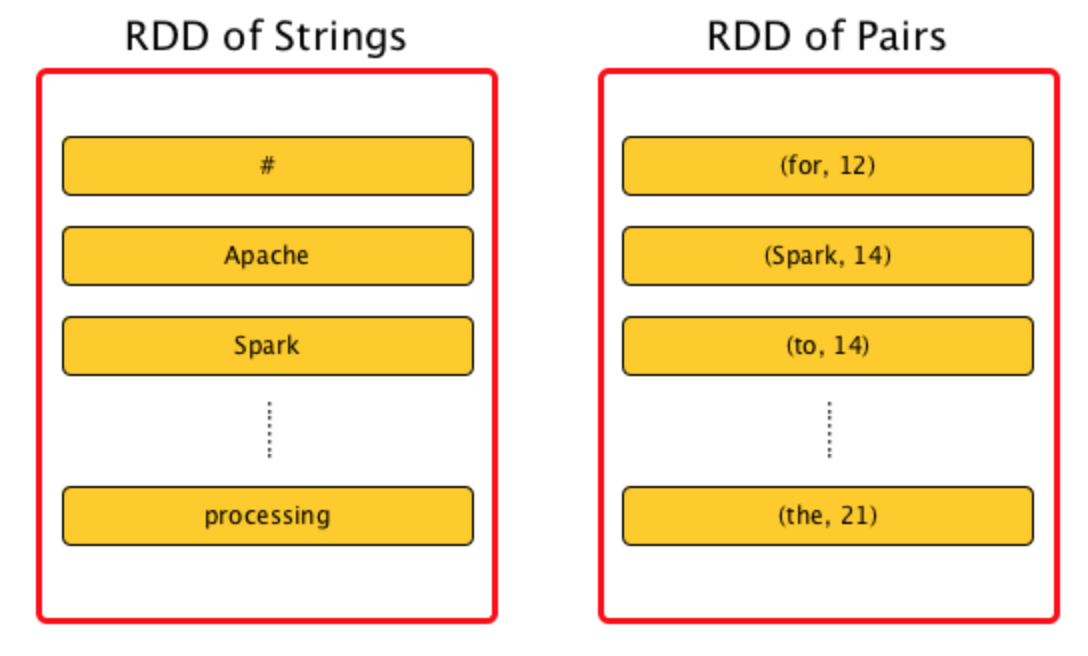
\includegraphics[scale=0.4]{RDD.png}
\caption{RDD結構}
\end{figure}

\begin{figure}[h]
\centering
\graphicspath{{/Users/FUDA/Documents/latex/masterThesis/image/}}
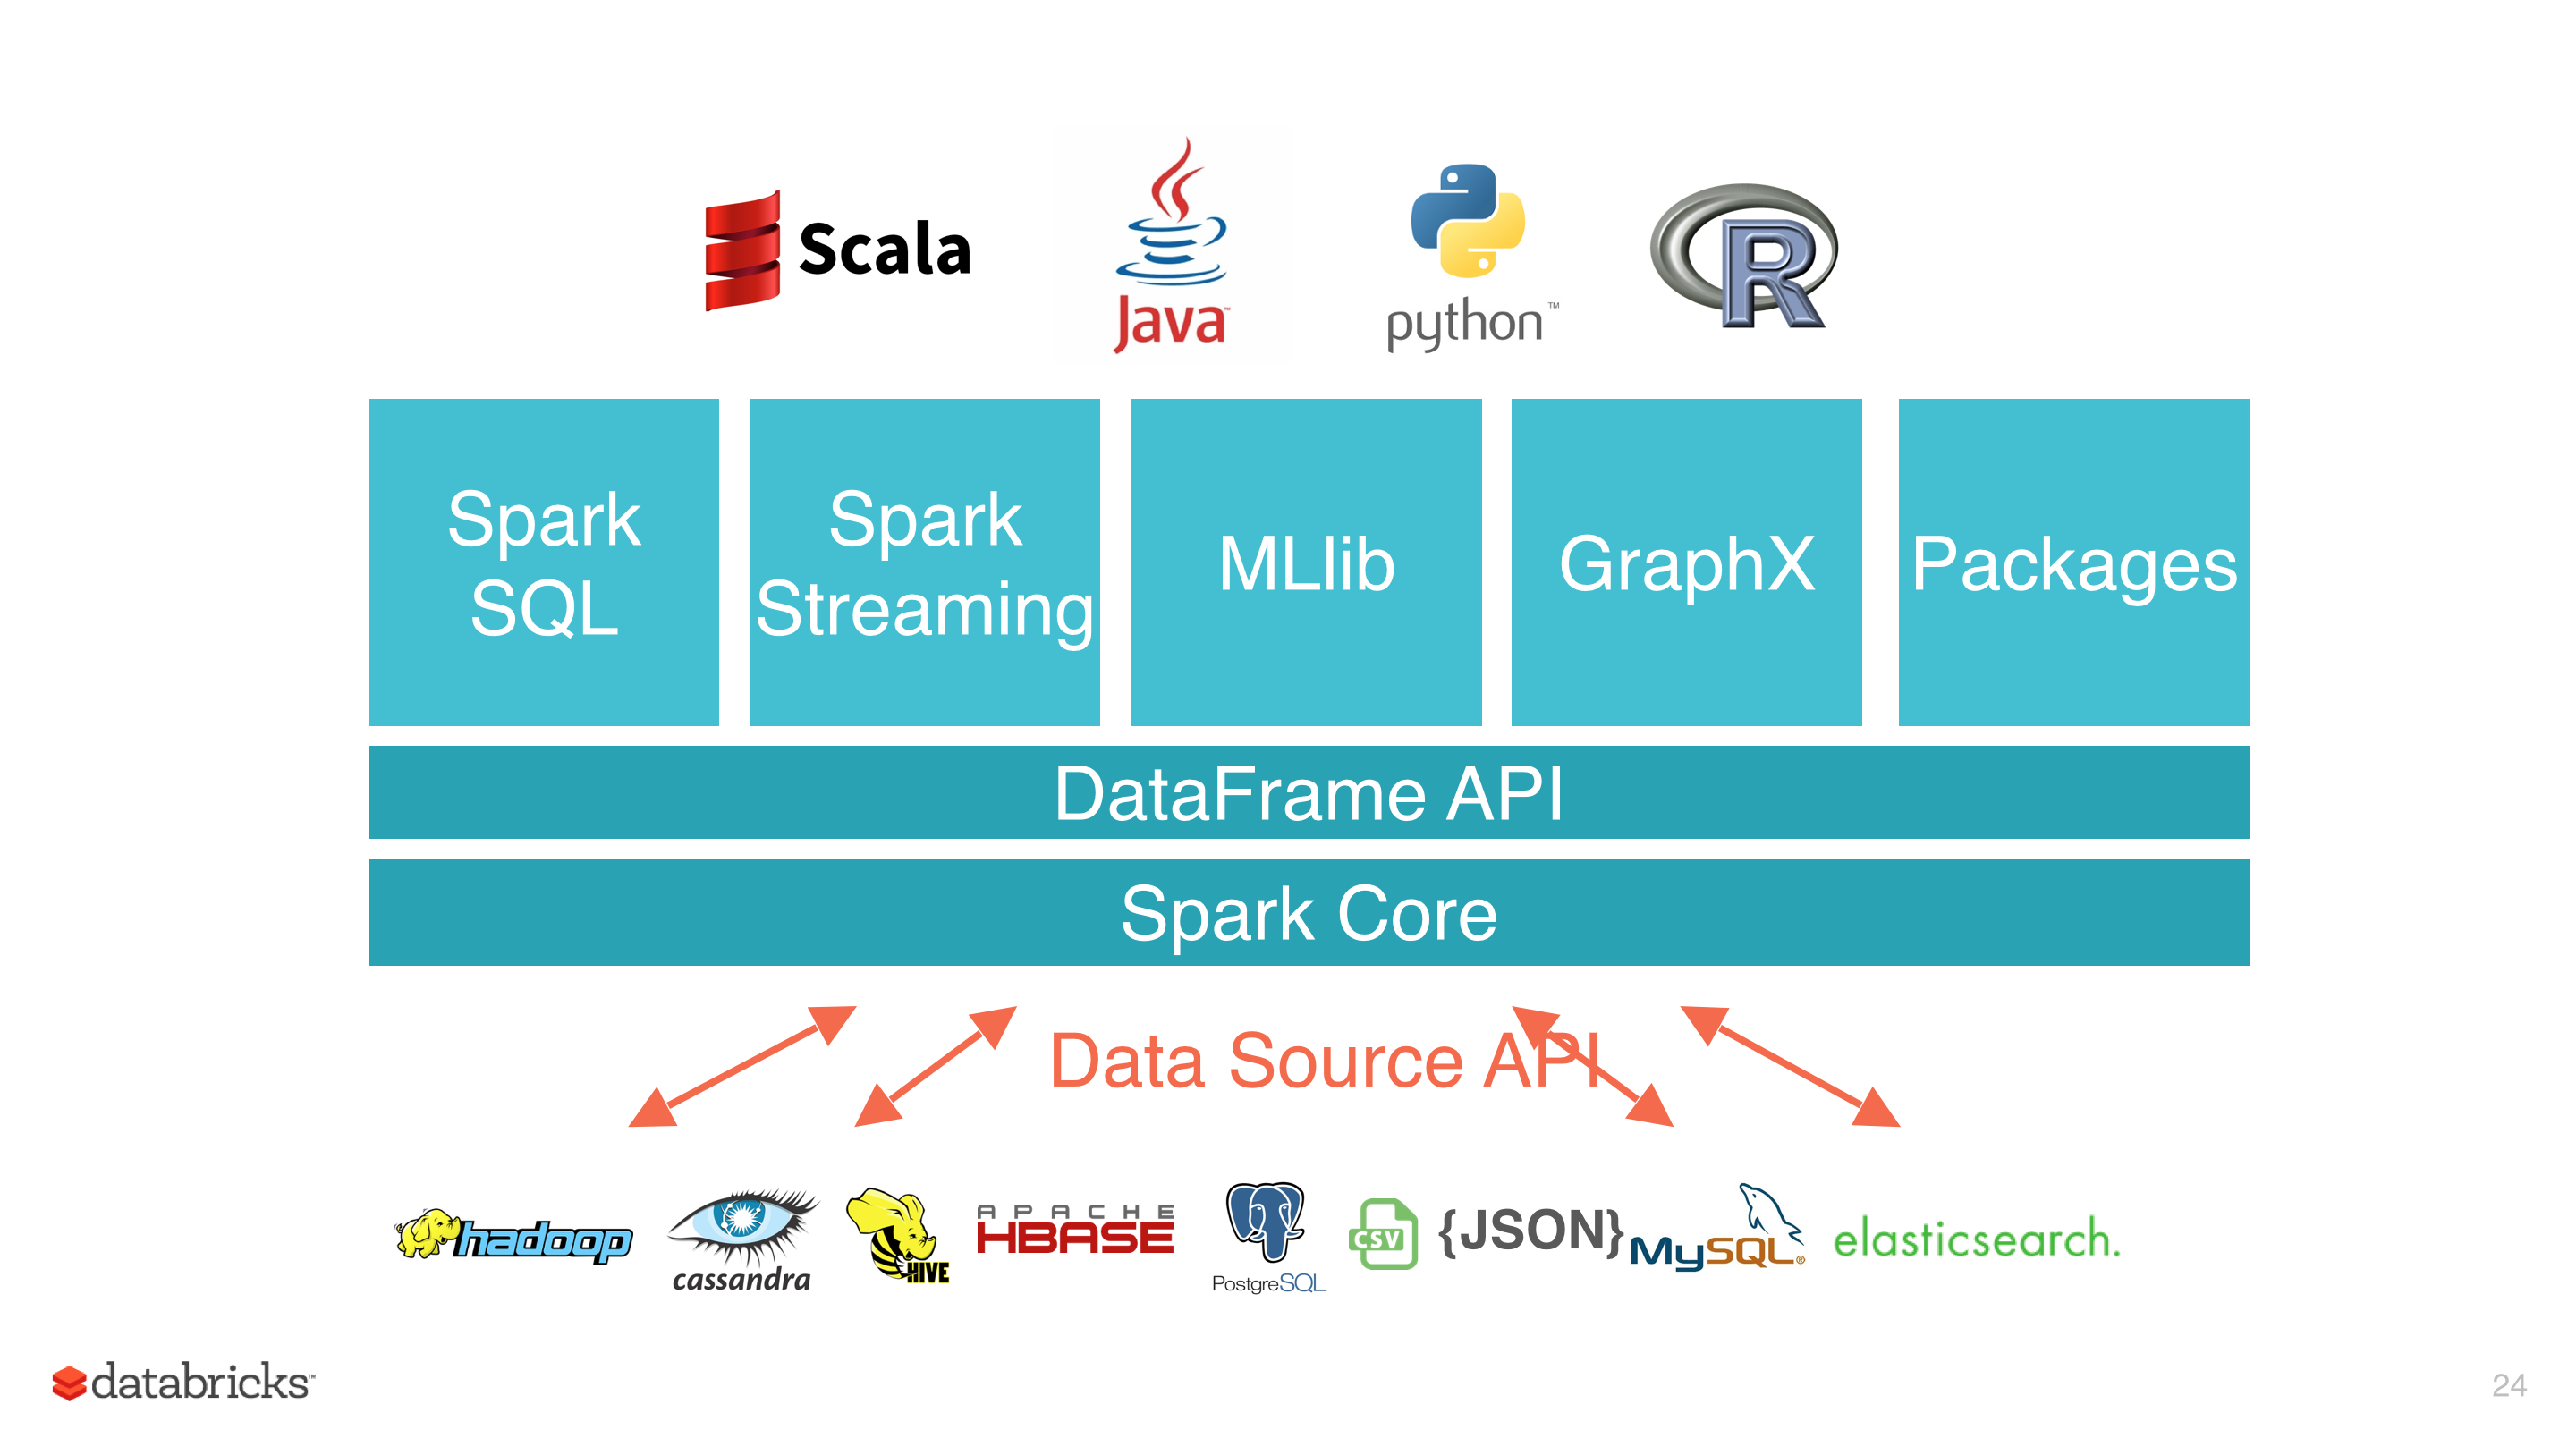
\includegraphics[scale=0.4]{spark.png}
\caption{Apache Spark 核心架構}
\end{figure}
\newpage
Apache Spark 有著豐富的函數庫,也針對Python, Java, Scala, R等程式語言提供一致的 API,核心架構如Fig.2,下面是 Apache Spark 所提供的API
\begin{itemize}
\item Spark Core
\item Spark SQL
\item Spark Streaming
\item MLlib
\item GraphX
\end{itemize}
Spark Core是整個Apache Spark的基礎,提供了分散式任務調度、排程和基本I/O ,而主要的程式抽象化結構RDD也是定義在這邊,RDD抽象化是經由Apache Spark 所支援的程式語言整合API呈現的,簡化了寫程式的複雜性。\\\par
Spark SQL 在Spark Core上定義了一個叫做 SchemaRDD的資料抽象化概念,提供結構化和半結構化資料的相關支援,另外Spark SQL允許使用者使用SQL遠法做資料查詢,也允許程式開發人員將SQL查詢與其他RDD所支援的資料處理方式一起使用。\\\par
Spark Streaming 是在處理即時串流資料的元件,例如web server所產生的紀錄,或是服務狀態的改變,Spark Streaming 擷取了微批次(micro batch)的資料並對資料執行RDD的轉換。\\\par
MLlib是Apache Spark 所提供的機器學習(Machine Learning)函數庫,MLlib可以使用許多常見的機器學習和統計學的演算法,大幅度簡化了機器學習的時間,其中有:
\begin{itemize}
\item 匯總統計:相關性、分層抽樣、假設檢定、亂數據產生
\item 分類與回歸:支援向量機(Support Vector Machine,簡稱SVM)、迴歸、線性迴歸、邏輯迴歸、決策樹(Decision Tree)、樸素貝葉斯(Naive Bayes)
\item 協同過濾:ALS 
\item 分群:K平均演算法(K-means)
\item 維度縮減:奇異值分解(Singular Value Decomposition,簡稱SVD),主成份分析(Principai Components Analysis,簡稱PCA)
\item 最佳化:隨機梯度下降(Stochastic Gradient Descent,簡稱SGD),L-BFGS
\end{itemize}
GraphX是Apache Spark 上的分散式圖形處理框架,此框架可用於表達圖形計算並可以類比Pregel抽象化,GraphX提供了許多處理圖像的操作,例如subgraph和mapVertices以及常見的圖形演算法。
\subsection{大數據}
所謂的大數據\cite{bigdata}是指無法以人工管理或是處理的資料集,也可以定義為多來源的結構化或非結構化的資料,而在大數據當中,我們常常用"5V"來描述大數據的特性,這5V分別是規模性(Volume)、價值(Value)、真實性(Veracity)、時效性(Velocity)及多樣性(Variety)。\\\par
5V當中,Volume所代表的是大數據的規模,也就是大數據以傳統的儲存方式已經無法負荷此龐大的資料量或是傳統的資料處 理方式已無法對其做運算了;Value是指大數據透過處理後所得到的資料產生的價值;Veracity是指資料的品質,可信度,資料是否可靠,或是結構的完整性;Velocity是指大數據資料產生的速度;Variety是指大數據的資料多樣性,在設計有關大數據的應用的時候,藉由上面五個的特性有助於檢視大數據的特徵。\\\par
而在這5V當中,本研究所要探討的是真實度Veracity在XML文件的建模與應用,在陳宇威學者的論文\cite{veracitymodel}當中有提到,大數據可以由兩個面向來討論,一個是資料理解性,一個是大數據的評價基準,而本研究所針對資料理解性面向進行建模,假設有n份基準XML文件以及m份被測量XML文件,使用者可以從多個角度對於XML文件進行真實度計分,XML文件真實度包含的面向極廣,對於真實度的定義每一個人不盡相同,所以本研究建構一個在Apache Spark 叢集上的Veracity真實度模型,使用物件導向程式設計(Object-Oriented Programming,簡稱OOP)的觀念,設計一個維度、屬性以及評分的抽象類別,將基本架構定義完整,做成Veracity Model API且是跑在 Apache Spark 叢集上,將實作細節交給使用者來決定,前面有提到使用者可以從不同的角度來評價XML的真實度評分,以及決定真實度要有多少維度以及多少屬性。並且本研究的模型應用在串流XML上,有別於以往傳統批次文件的處理方式,串流的資料處理方式更符合現代的資料處理架構及場景,針對一個大數據串流XML真實度評價模型是一個除了評價資料真實度之外,也可以篩選真實度較高之資料的解決方案。
